%%%
 %
 % Copyright (C) 2019 Ángel Iván Gladín García
 %
 % This program is free software: you can redistribute it and/or modify
 % it under the terms of the GNU General Public License as published by
 % the Free Software Foundation, either version 3 of the License, or
 % (at your option) any later version.
 %
 % This program is distributed in the hope that it will be useful,
 % but WITHOUT ANY WARRANTY; without even the implied warranty of
 % MERCHANTABILITY or FITNESS FOR A PARTICULAR PURPOSE.  See the
 % GNU General Public License for more details.
 %
 % You should have received a copy of the GNU General Public License
 % along with this program.  If not, see <http://www.gnu.org/licenses/>.
%%%

%%%%%%%%%%%%%%%%%%%%%%%%%%%%%%%%%%%%%%%%%%%%%%%%%%%%%%%%%%%%%%%%%%%%%%%%%%%%%%%%%%%%%%%%%
\documentclass[11pt,letterpaper]{article}
\usepackage[utf8]{inputenc}
\usepackage[spanish]{babel}
\usepackage[margin=1in]{geometry}
 
\usepackage{listings}
\usepackage{color}
\usepackage{graphicx}
\usepackage{enumerate}
\usepackage{enumitem}

\usepackage{longtable}
\usepackage{hyperref}
\usepackage{commath}

\usepackage{minted}
\usemintedstyle{emacs}


\usepackage{bbm}
\usepackage{dsfont}
\usepackage{mathrsfs}
\usepackage{amsmath,amsthm,amssymb}
\usepackage{mathtools}
\usepackage{longtable}
%%%%%%%%%%%%%%%%%%%%%%%%%%%%%%%%%%%%%%%%%%%%%%%%%%%%%%%%%%%%%%%%%%%%%%%%%%%%%%%%%%%%%%%%%

\renewcommand{\theenumi}{\alph{enumi}}

%%%%%%%%%%%%%%%%%%%%%%%%%%%%%%%%%%%%%%%%%%%%%%%%%%%%%%%%%%%%%%%%%%%%%%%%%%%%%%%%%%%%%%%%%
\newcommand{\Z}{\mathbb{Z}}
\newcommand{\N}{\mathbb{N}}
\newcommand{\Q}{\mathbb{Q}}
\newcommand{\R}{\mathbb{R}}
\newcommand{\Oh}{\mathcal{O}} %% Notacion "O"
\newcommand{\ent}{\Longrightarrow}
\newcommand{\lra}{\longrightarrow}
\newcommand{\ra}{\rightarrow}
\newcommand{\sii}{\Longleftrightarrow}
\newcommand{\clase}[1]{\overline{#1}}  %% barrita sobre letras
\newcommand{\ord}{\text{ord}}
\newcommand{\leg}[2]{\left( \frac{#1}{#2}\right)} %% Simbolo de Legendre
\newcommand{\sol}{\textbf{\underline{Solución}: }} %% Solución

%%%%%%%%%%%%%%%%%%%%%%%%%%%%%%%%%%%%%%%%%%%%%%%%%%%%%%%%%%%%%%%%%%%%%%%%%%%%%%%%%%%%%%%%%

\begin{document}

%%%%%%%%%%%%%%%%%%%%%%%%%%%%%%%%%%%%%%%%%%%%%%%%%%%%%%%%%%%%%%%%%%%%%%%%%%%%%%%%%%%%%%%%%
\title{
    \vspace{-2cm}
        Universidad Nacional Autónoma de México\\
        Facultad de Ciencias\\
        Criptografía y Seguridad\\
    \vspace{.5cm}
    \large
        \textbf{Tarea 2}\\        
}
\author{
    Ángel Iván Gladín García\\
    No. cuenta: 313112470\\
    \texttt{angelgladin@ciencias.unam.mx}
}
\date{29 de Abril 2019}
\maketitle
%%%%%%%%%%%%%%%%%%%%%%%%%%%%%%%%%%%%%%%%%%%%%%%%%%%%%%%%%%%%%%%%%%%%%%%%%%%%%%%%%%%%%%%%%

%%%%%%%%%%%%%%%%%%%%%%%%%%%%%%%%%%%%%%%%%%%%%%%%%%%%%%%%%%%%%%%%%%%%%%%%%%%%%%%%%%%%%%%%%
\newtheorem{theorem}{Teorema}
\newtheorem{example}{Ejemplo}
\newtheorem{corollary}{Corolario}
\newtheorem{lemma}{Lemma}
\newtheorem{definition}{Definición}
\newtheorem{prop}{Proposición}
%%%%%%%%%%%%%%%%%%%%%%%%%%%%%%%%%%%%%%%%%%%%%%%%%%%%%%%%%%%%%%%%%%%%%%%%%%%%%%%%%%%%%%%%%


%%%%%%%%%%%%%%%%%%%%%%%%%%%%%%%%%%%%%%%%%%%%%%%%%%%%%%%%%%%%%%%%%%%%%%%%%%%%%%%%%%%%%%%%%

%%%%%%%%
\section{Sea $\Z_{89627}$}

\begin{enumerate}[label=\alph*)]
\item Muestre que $2$ es generardor de $\Z^*_{89627}$.\\
\sol Se procederá a dar la la definición de generador:
\begin{definition}
Una unidad $g \in \Z_{n}^{*}$ es llamado un \textbf{generador} o \textbf{raíz primitiva} de
$\Z_{n}^{*}$ si cada $a \in \Z_{n}^{*}$ se tiene $g^k = a$ para algún entero $k$.
\end{definition}
Teniendo esa definición se hizo un programa en Python para dado un generador $g$ y $p$ primo 
tal que $|\Z_p| = p$ verificar si $g$ genera a $\Z_{n}^{*}$.

\begin{minted}{python}
# Generador del grupo
g = 2
# Orden del grupo
p = 89627

def g_es_generador(g, p):
    # Se crea conjunto para no tener repetidos y se guardarán los elementos de Z_p
    s = set()
    # Se itera de 1 hasta p-1 las potencias denotado por k
    for k in range(p):
        # Agregamos g^k mod p al conjunto
        s.add(pow(g, k, p))
    # Regresamos la cardinalidad del conjunto.
    return len(s)

# Verificamos si en efecto es un generador
print(g_es_generador(g, p) == p-1)
\end{minted}

Con el \textit{script} previo se puede corroborar que en efecto $2$ genera a $\Z_{n}^{*}$.

\item Mediante cálculo de índices encontrar $\log_2 (88777)$.\\
\sol 
\begin{figure}[H]
\caption{Algoritmo de cálculo de índices para logaritmos discretos en grupos cíclicos.}
\centering
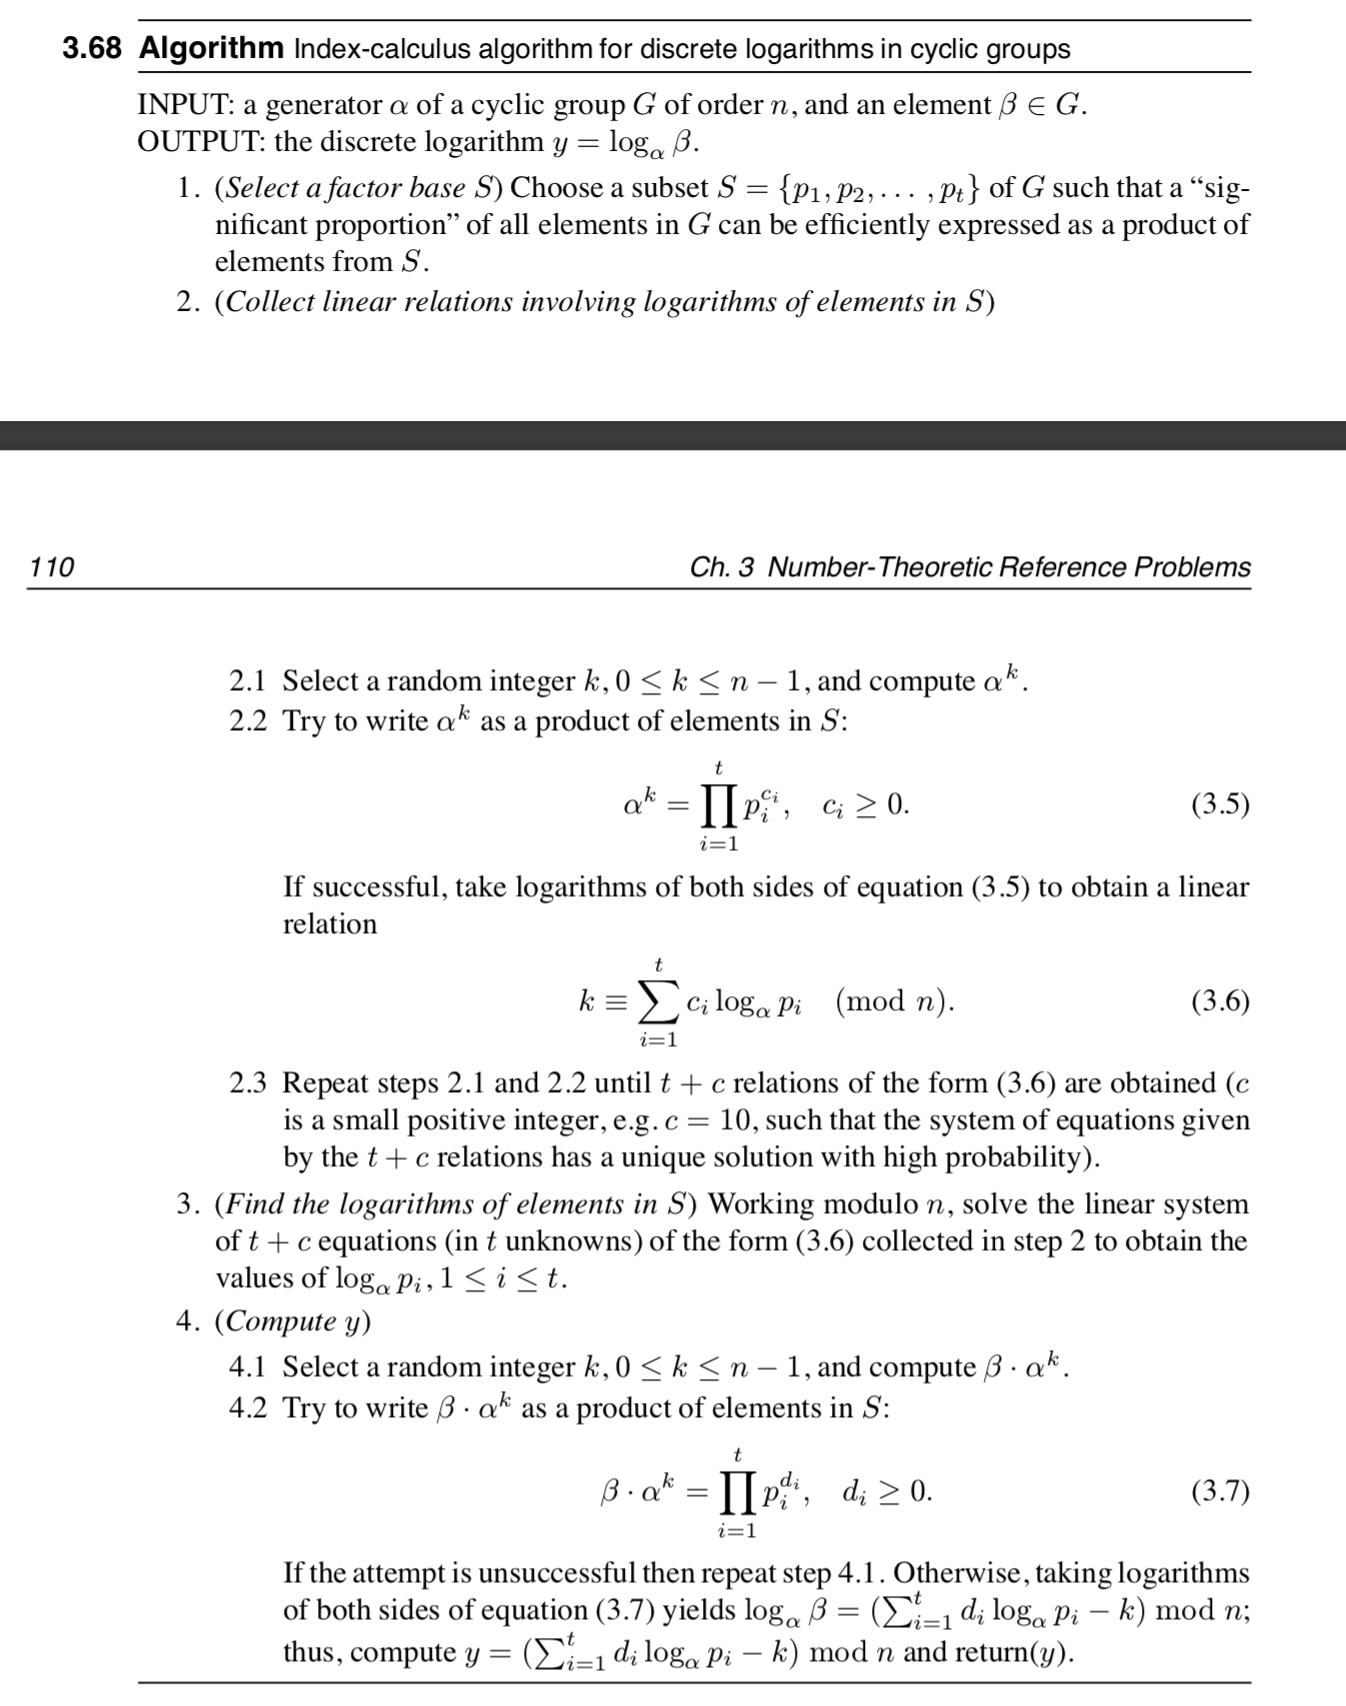
\includegraphics[width=0.9\textwidth]{assets/poi.png}
\end{figure}

Con ayuda de un programa que encontré en internet 
\url{https://github.com/simonedaniello/Index-Calculus-in-C} verifiqué que 
$\log_2 88777= 137$ en $\Z_{89267}^*$.


\item Mediante paso grande paso chico encontrar $\log_2 (88777)$.\\
\sol Se realizo un programa en \textit{Python} siguiendo el algoritmo descrito abajo para facilitar 
las cuentas:

\begin{minted}{python}
from math import ceil, sqrt


def bsgs(g, beta, p):
    # Raíz de p
    M = ceil(sqrt(p - 1))

    # La tabla con las entradas (alpha^j, j)
    tabla = {pow(g, j, p): j for j in range(M)}

    # alpha^{-m}
    c = pow(g, M * (p - 2), p)

    for j in range(M):
        gamma = (beta * pow(c, j, p)) % p
        if gamma in tabla:
            return j * M + tabla[gamma]

    # No se encontró solución.
    return None

# Generador del grupo
g = 2
# Beta
beta = 88777
# Orden del grupo más uno
p = 89627

print(bsgs(g, beta, p))
\end{minted}


\begin{figure}[h]
\caption{Algoritmo de paso grande paso chico}
\centering
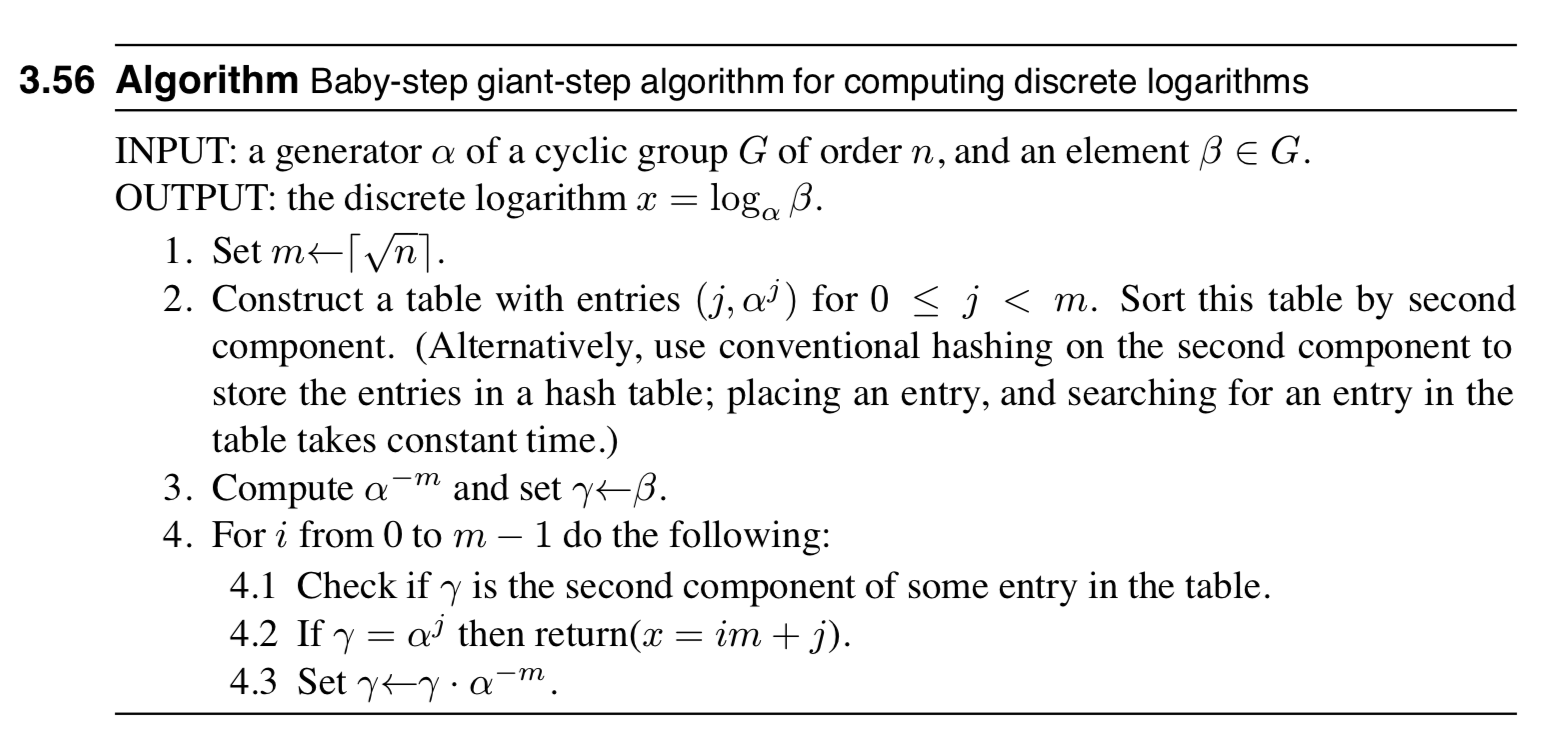
\includegraphics[width=0.9\textwidth]{assets/3b.png}
\end{figure}

\underline{Ejecución del algoritmo:}
\begin{itemize}
\item Sea $m \leftarrow 300$.
\item Construir una tabla con las entradas $(j, \alpha^j)$, (en el programa se hizo al revez).
\begin{table}[H]
\begin{longtable}{|l|l|l|l|}
\hline
"1":     0 & "2817":  201 & "49779": 181, & "70752": 69 \\ \hline 
"1024":  10 & "28254": 72 & "49951": 88, & "70843": 250 \\ \hline
"10275": 89 & "28365": 108 & "50238": 44, & "7101": 297 \\ \hline
"1034":  207 & "28404": 299 & "50329": 262, & "71462": 22 \\ \hline
"10364": 30 & "28982": 253 & "50763": 237, & "71814": 37 \\ \hline
"10849": 45 & "29371": 283 & "50859": 293, & "72139": 57 \\ \hline
"10968": 275 & "29498": 106 & "50915": 157, & "72202": 82 \\ \hline
"11031": 263 & "30211": 95 & "512": 9, & "72919": 217 \\ \hline
"11130": 242 & "30796": 131 & "51281": 145, & "72998": 197 \\ \hline
"11268": 203 & "3106": 222 & "51337": 101, & "73500": 41 \\ \hline
"11410": 113 & "31154": 258 & "517": 206, & "74563": 281 \\ \hline
"11899": 238 & "31217": 97 & "51740": 148, & "74773": 93 \\ \hline
"12091": 294 & "31432": 79 & "5182": 29, & "75438": 169 \\ \hline
"12203": 158 & "31988": 163 & "51877": 70, & "76027": 141 \\ \hline
"12424": 224 & "32": 5 & "52059": 251, & "76153": 19 \\ \hline
"128":   7 & "32330": 123 & "52188": 104, & "76197": 34 \\ \hline
"12935": 146 & "32768": 15 & "52602": 256, & "76345": 194 \\ \hline
"13047": 102 & "32780": 190 & "52896": 121, & "76650": 166 \\ \hline
"13224": 119 & "32871": 171 & "53297": 23, & "7699": 129 \\ \hline
"1371":  272 & "3306": 117 & "54001": 38, & "77801": 175 \\ \hline
"13853": 149 & "33088": 212 & "54651": 58, & "78120": 230 \\ \hline
"14127": 71 & "33557": 133 & "54777": 83, & "78287": 50 \\ \hline
"14202": 298 & "33934": 25 & "5484": 274, & "7858": 77 \\ \hline
"14491": 252 & "34989": 260 & "55412": 151, & "78595": 269 \\ \hline
"14749": 105 & "35227": 143 & "5565": 241, & "78700": 61 \\ \hline
"15398": 130 & "35241": 99 & "55714": 286, & "79386": 126 \\ \hline
"1553":  221 & "35376": 68 & "56211": 218, & "79448": 185 \\ \hline
"15577": 257 & "35731": 21 & "5634": 202, & "79665": 179 \\ \hline
"15716": 78 & "35907": 36 & "56369": 198, & "79708": 86 \\ \hline
"15994": 162 & "36101": 81 & "56508": 73, & "79911": 235 \\ \hline
"16":    4 & "36499": 196 & "56730": 109, & "79935": 291 \\ \hline
"16165": 122 & "36750": 40 & "5705": 112, & "79949": 155 \\ \hline
"16384": 14 & "37719": 168 & "57373": 42, & "7997": 161 \\ \hline
"16390": 189 & "38325": 165 & "57964": 254, & "8": 3 \\ \hline
"1653":  116 & "39060": 229 & "58742": 284, & "80235": 249 \\ \hline
"16544": 211 & "3929": 76 & "58996": 107, & "80883": 56 \\ \hline
"16967": 24 & "39350": 60 & "59499": 282, & "81273": 216 \\ \hline
"17688": 67 & "39693": 125 & "59919": 94, & "8192": 13 \\ \hline
"18375": 39 & "39724": 184 & "60422": 96, & "8195": 188 \\ \hline
"19530": 228 & "39854": 85 & "61249": 170, & "82095": 280 \\ \hline
"19675": 59 & "4": 2 & "61592": 132, & "82200": 92 \\ \hline
"19862": 183 & "4096": 12 & "6212": 223, & "8272": 210 \\ \hline
"19927": 84 & "41100": 91 & "62308": 259, & "82827": 140 \\ \hline
"2":     1 & "4136": 209 & "62427": 142, & "82890": 18 \\ \hline
"2048":  11 & "41445": 17 & "62434": 98, & "82912": 33 \\ \hline
"20550": 90 & "41456": 32 & "62679": 20, & "82986": 193 \\ \hline
"2068":  208 & "41493": 192 & "62767": 35, & "83714": 174 \\ \hline
"20728": 31 & "41857": 173 & "62864": 80, & "83957": 49 \\ \hline
"21197": 152 & "42323": 177 & "63063": 195, & "84111": 268 \\ \hline
"21698": 46 & "42394": 153 & "63673": 167, & "84646": 178 \\ \hline
"21801": 287 & "42725": 214 & "63976": 164, & "84769": 234 \\ \hline
"21936": 276 & "43396": 47 & "64": 6, & "84781": 290 \\ \hline
"22062": 264 & "43599": 232 & "64660": 124, & "84788": 154 \\ \hline
"2211":  64 & "43602": 288 & "65536": 16, & "84931": 248 \\ \hline
"22260": 243 & "43872": 277 & "65560": 191, & "85255": 55 \\ \hline
"22536": 204 & "44124": 265 & "65742": 172, & "85450": 215 \\ \hline
"22795": 219 & "4422": 65 & "65975": 176, & "85861": 279 \\ \hline
"22820": 114 & "44267": 52 & "6612": 118, & "86227": 139 \\ \hline
"23111": 199 & "44520": 244 & "66176": 213, & "86792": 48 \\ \hline
"23389": 74 & "44601": 135 & "66613": 231, & "86869": 267 \\ \hline
"23798": 239 & "45072": 205 & "66947": 51, & "87198": 233 \\ \hline
"23833": 110 & "45499": 271 & "67114": 134, & "87204": 289 \\ \hline
"24182": 295 & "45590": 220 & "67563": 270, & "87279": 247 \\ \hline
"24406": 159 & "45640": 115 & "67773": 62, & "87441": 54 \\ \hline
"24848": 225 & "45919": 63 & "67868": 26, & "87744": 278 \\ \hline
"25119": 43 & "46109": 27 & "69145": 127, & "87927": 138 \\ \hline
"256":   8 & "46222": 200 & "69269": 186, & "88248": 266 \\ \hline
"25870": 147 & "46778": 75 & "69703": 180, & "8844": 66 \\ \hline
"2591":  28 & "47596": 240 & "69789": 87, & "88453": 246 \\ \hline
"26094": 103 & "47666": 111 & "69978": 261, & "88534": 53 \\ \hline
"26301": 255 & "48364": 296 & "70195": 236, & "88777": 137 \\ \hline
"26448": 120 & "48663": 128 & "70243": 292, & "89040": 245 \\ \hline
"2742":  273 & "48812": 160 & "70271": 156, & "89202": 136 \\ \hline
"27706": 150 & "48911": 187 & "70454": 144, & "9765": 227 \\ \hline
"27857": 285 & "49696": 226 & "70482": 100, & "9931": 18 \\ \hline 
\end{longtable}
\end{table}
\item Calcular $\alpha^{-m} = 59166$
\item Regresar $x = im + j = 137$
\end{itemize}
Por tanto $\log_2 88777= 137$ en $\Z_{89267}^*$.

\item Mediante $\rho$-Pollard para logaritmos encontrar $\log_2 (88777)$.\\
\sol 
\begin{figure}[H]
\caption{Algoritmo de la Rho de Pollard para calcular logaritmo discreto}
\centering
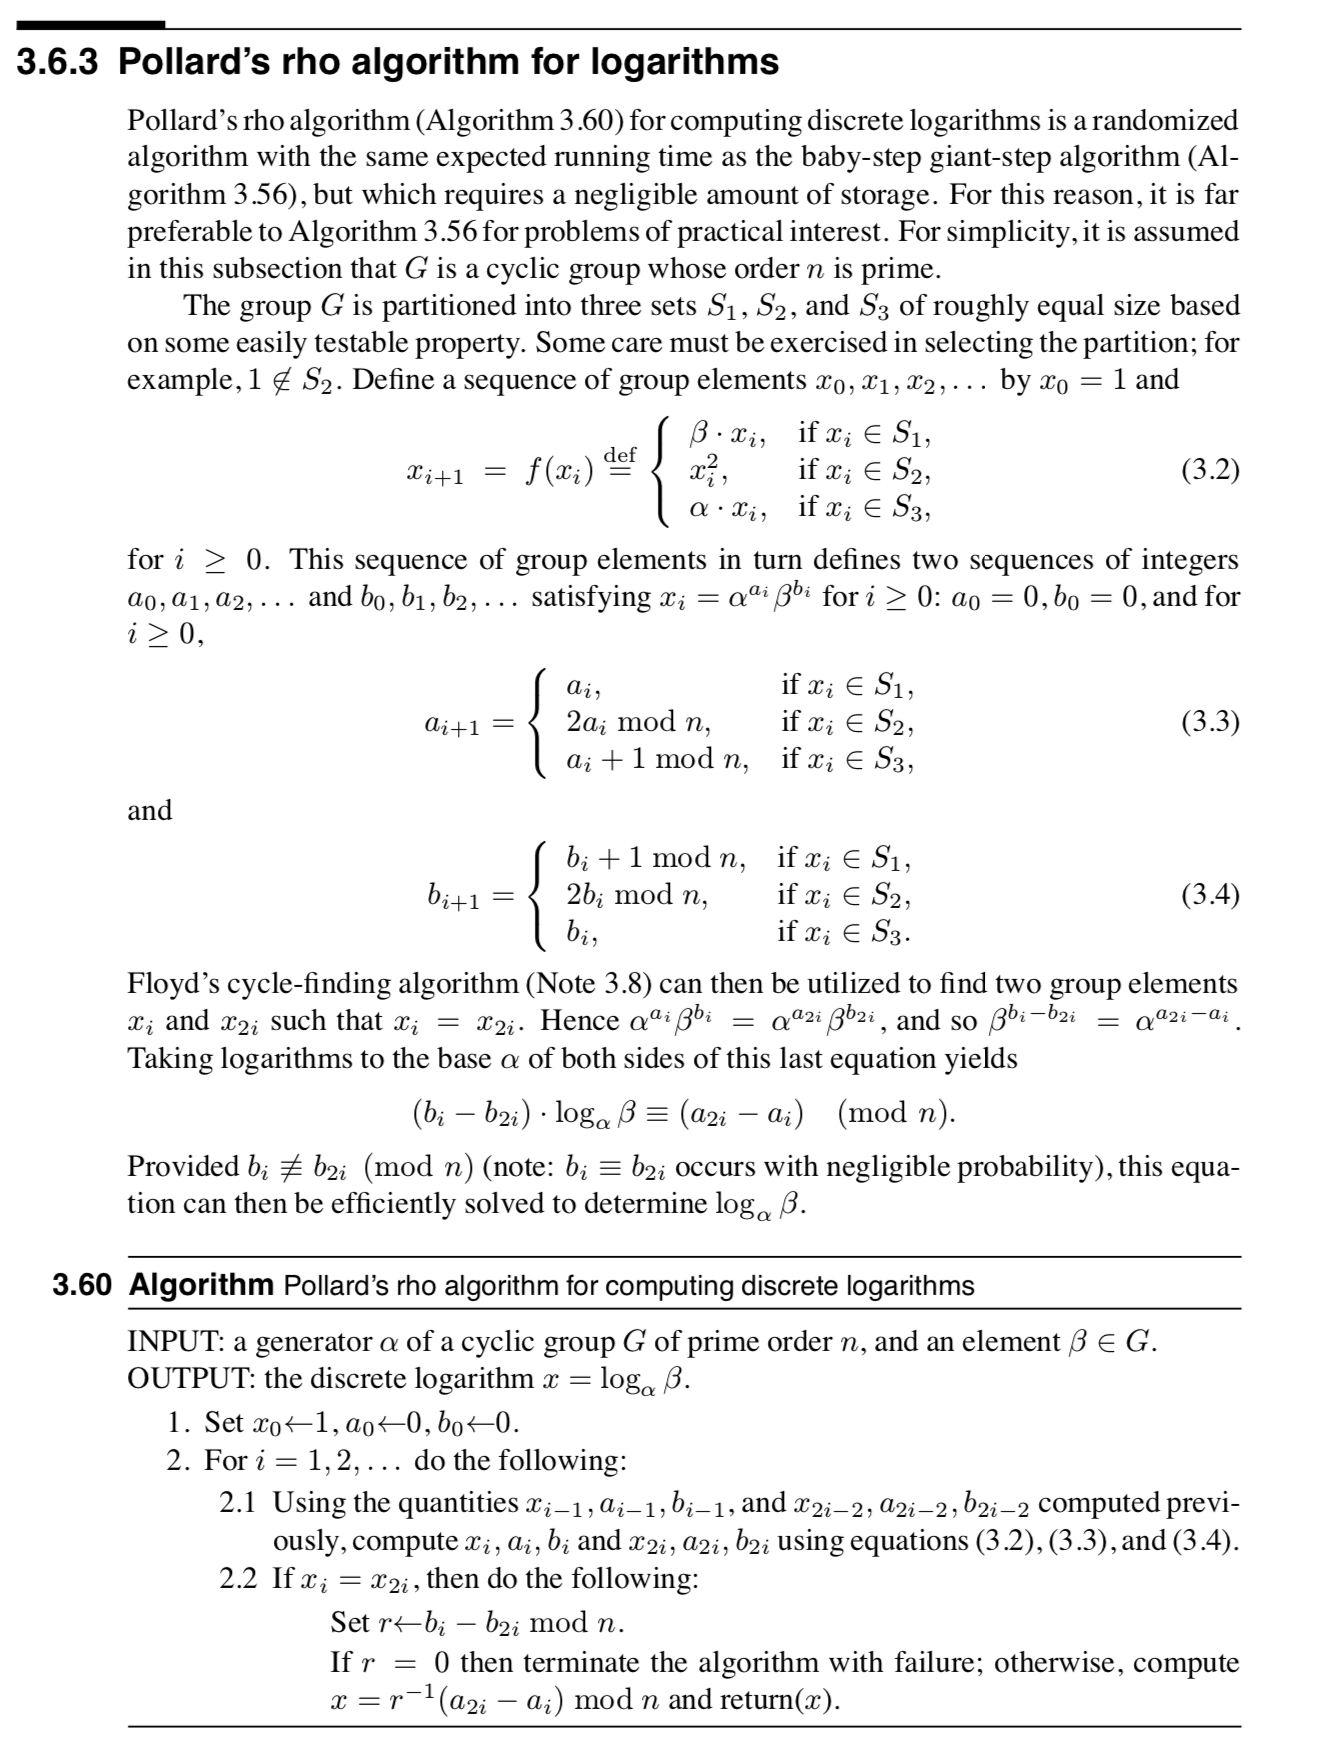
\includegraphics[width=0.9\textwidth]{assets/1d.png}
\end{figure}

Script en Python que hace $\rho$-Pollard.

\begin{minted}{python}
def ext_euclid(a, b):
    if b == 0:
        return a, 1, 0
    else:
        d, xx, yy = ext_euclid(b, a % b)
        x = yy
        y = xx - (a / b) * yy
        return d, x, y


def inverse(a, n):
    return ext_euclid(a, n)[1]


def xab(x, a, b, (G, H, P, Q)):
    sub = x % 3

    if sub == 0:
        x = x * G % P
        a = (a + 1) % Q

    if sub == 1:
        x = x * H % P
        b = (b + 1) % Q

    if sub == 2:
        x = x * x % P
        a = a * 2 % Q
        b = b * 2 % Q

    return x, a, b

def pollard(G, H, P):
    Q = (P - 1) / 2

    x = G * H
    a = 1
    b = 1

    X = x
    A = a
    B = b

    for i in range(1, P):
        # Tortuga
        x, a, b = xab(x, a, b, (G, H, P, Q))

        # Liebre
        X, A, B = xab(X, A, B, (G, H, P, Q))
        X, A, B = xab(X, A, B, (G, H, P, Q))

        if x == X:
            break

    nom = a - A
    denom = B - b

    res = (inverse(denom, Q) * nom) % Q

    if pow(G, res, P) == H:
        return res

    return res + Q


generador = 2
beta = 88777
p = 89627

res = pollard(generador, beta, p)
print(res)

\end{minted}

Por tanto $\log_2 88777= 137$ en $\Z_{89267}^*$.

\item Con el método de su preferencia calcular $\log_2 (54539)$.\\
\sol Usando el algoritmo de paso chico paso grande queda como:\\
\underline{Ejecución del algoritmo:}

\begin{itemize}
\item Sea $m \leftarrow 300$.

\begin{table}[H]
\begin{longtable}{|l|l|l|l|l|}
\hline
"1": 0        & "23798": 239   &  "41456": 32   & "56730": 109  & "76197": 34  \\ \hline
"1024": 10    & "23833": 110   &  "41493": 192  & "5705": 112   & "76345": 194 \\ \hline
"10275": 89   & "24182": 295   &  "41857": 173  & "57373": 42   & "76650": 166 \\ \hline
"1034": 207   & "24406": 159   &  "42323": 177  & "57964": 254  & "7699": 129  \\ \hline
"10364": 30   & "24848": 225   &  "42394": 153  & "58742": 284  & "77801": 175 \\ \hline
"10849": 45   & "25119": 43    &  "42725": 214  & "58996": 107  & "78120": 230 \\ \hline
"10968": 275  & "256": 8       &  "43396": 47   & "59499": 282  & "78287": 50  \\ \hline
"11031": 263  & "25870": 147   &  "43599": 232  & "59919": 94   & "7858": 77   \\ \hline
"11130": 242  & "2591": 28     &  "43602": 288  & "60422": 96   & "78595": 269 \\ \hline
"11268": 203  & "26094": 103   &  "43872": 277  & "61249": 170  & "78700": 61  \\ \hline
"11410": 113  & "26301": 255   &  "44124": 265  & "61592": 132  & "79386": 126 \\ \hline
"11899": 238  & "26448": 120   &  "4422": 65    & "6212": 223   & "79448": 185 \\ \hline
"12091": 294  & "2742": 273    &  "44267": 52   & "62308": 259  & "79665": 179 \\ \hline
"12203": 158  & "27706": 150   &  "44520": 244  & "62427": 142  & "79708": 86  \\ \hline
"12424": 224  & "27857": 285   &  "44601": 135  & "62434": 98   & "79911": 235 \\ \hline
"128": 7      & "2817": 201    &  "45072": 205  & "62679": 20   & "79935": 291 \\ \hline
"12935": 146  & "28254": 72    &  "45499": 271  & "62767": 35   & "79949": 155 \\ \hline
"13047": 102  & "28365": 108   &  "45590": 220  & "62864": 80   & "7997": 161  \\ \hline
"13224": 119  & "28404": 299   &  "45640": 115  & "63063": 195  & "8": 3       \\ \hline
"1371": 272   & "28982": 253   &  "45919": 63   & "63673": 167  & "80235": 249 \\ \hline
"13853": 149  & "29371": 283   &  "46109": 27   & "63976": 164  & "80883": 56  \\ \hline
"14127": 71   & "29498": 106   &  "46222": 200  & "64": 6       & "81273": 216 \\ \hline
"14202": 298  & "30211": 95    &  "46778": 75   & "64660": 124  & "8192": 13   \\ \hline
"14491": 252  & "30796": 131   &  "47596": 240  & "65536": 16   & "8195": 188  \\ \hline
"14749": 105  & "3106": 222    &  "47666": 111  & "65560": 191  & "82095": 280 \\ \hline
"15398": 130  & "31154": 258   &  "48364": 296  & "65742": 172  & "82200": 92  \\ \hline
"1553": 221   & "31217": 97    &  "48663": 128  & "65975": 176  & "8272": 210  \\ \hline
"15577": 257  & "31432": 79    &  "48812": 160  & "6612": 118   & "82827": 140 \\ \hline
"15716": 78   & "31988": 163   &  "48911": 187  & "66176": 213  & "82890": 18  \\ \hline
"15994": 162  & "32": 5        &  "49696": 226  & "66613": 231  & "82912": 33  \\ \hline
"16": 4       & "32330": 123   &  "49779": 181  & "66947": 51   & "82986": 193 \\ \hline
"16165": 122  & "32768": 15    &  "49951": 88   & "67114": 134  & "83714": 174 \\ \hline
"16384": 14   & "32780": 190   &  "50238": 44   & "67563": 270  & "83957": 49  \\ \hline
"16390": 189  & "32871": 171   &  "50329": 262  & "67773": 62   & "84111": 268 \\ \hline
"1653": 116   & "3306": 117    &  "50763": 237  & "67868": 26   & "84646": 178 \\ \hline
"16544": 211  & "33088": 212   &  "50859": 293  & "69145": 127  & "84769": 234 \\ \hline
"16967": 24   & "33557": 133   &  "50915": 157  & "69269": 186  & "84781": 290 \\ \hline
"17688": 67   & "33934": 25    &  "512": 9      & "69703": 180  & "84788": 154 \\ \hline
"18375": 39   & "34989": 260   &  "51281": 145  & "69789": 87   & "84931": 248 \\ \hline
"19530": 228  & "35227": 143   &  "51337": 101  & "69978": 261  & "85255": 55  \\ \hline
"19675": 59   & "35241": 99    &  "517": 206    & "70195": 236  & "85450": 215 \\ \hline
"19862": 183  & "35376": 68    &  "51740": 148  & "70243": 292  & "85861": 279 \\ \hline
"19927": 84   & "35731": 21    &  "5182": 29    & "70271": 156  & "86227": 139 \\ \hline
"2": 1        & "35907": 36    &  "51877": 70   & "70454": 144  & "86792": 48  \\ \hline
"2048": 11    & "36101": 81    &  "52059": 251  & "70482": 100  & "86869": 267 \\ \hline
"20550": 90   & "36499": 196   &  "52188": 104  & "70752": 69   & "87198": 233 \\ \hline
"2068": 208   & "36750": 40    &  "52602": 256  & "70843": 250  & "87204": 289 \\ \hline
"20728": 31   & "37719": 168   &  "52896": 121  & "7101": 297   & "87279": 247 \\ \hline
"21197": 152  & "38325": 165   &  "53297": 23   & "71462": 22   & "87441": 54  \\ \hline
"21698": 46   & "39060": 229   &  "54001": 38   & "71814": 37   & "87744": 278 \\ \hline
"21801": 287  & "3929": 76     &  "54651": 58   & "72139": 57   & "87927": 138 \\ \hline
"21936": 276  & "39350": 60    &  "54777": 83   & "72202": 82   & "88248": 266 \\ \hline
"22062": 264  & "39693": 125   &  "5484": 274   & "72919": 217  & "8844": 66   \\ \hline
"2211": 64    & "39724": 184   &  "55412": 151  & "72998": 197  & "88453": 246 \\ \hline
"22260": 243  & "39854": 85    &  "5565": 241   & "73500": 41   & "88534": 53  \\ \hline
"22536": 204  & "4": 2         &  "55714": 286  & "74563": 281  & "88777": 137 \\ \hline
"22795": 219  & "4096": 12     &  "56211": 218  & "74773": 93   & "89040": 245 \\ \hline
"22820": 114  & "41100": 91    &  "5634": 202   & "75438": 169  & "89202": 136 \\ \hline
"23111": 199  & "4136": 209    &  "56369": 198  & "76027": 141  & "9765": 227  \\ \hline
"23389": 74   & "41445": 17    &  "56508": 73   & "76153": 19   & "9931": 182  \\ \hline
\end{longtable}
\end{table}

\item Calcular $\alpha^{-m} = 59166$.
\item Regresar $x = im + j = 953$.
\end{itemize}

Por tanto $\log_2 54539 = 953$ en $\Z_{89267}^*$.


\item Si los parámetros públicos son $(89627, 2, 88777)$, descifrar el siguiente mensaje el cual
está encriptado con Gamal justifica tu desifrado.\\
Si $\gamma = 54539$.
\begin{table}[H]
\centering
\begin{tabular}{lll}
($\gamma$, 81315)($\gamma$, 87570)  & ($\gamma$, 31275)($\gamma$, 50040) & ($\gamma$, 31275) \\
($\gamma$, 18764)($\gamma$, 500040) & ($\gamma$, 31275)($\gamma$, 50040) & ($\gamma$, 12510) \\
($\gamma$, 50040)($\gamma$, 68805)  &                                    &                  
\end{tabular}
\end{table}

\sol La llave pública $A$ es de la forma $(p, \alpha, \alpha^a)$, fijándose en el tercer parámetro
de la llave que es $88777$ la cual ya se había calculado su logaritmo (base 2) que corresponde con el
generador a la potencia $k$, es decir, sea $g$ un generador de de $\Z_{89627}^*$ y $k$ un natural,
entonces $g^k \in \Z_{89627}^*$. Por consiguiente $\alpha^a \mod{89627}$, que es $2^{137} \mod 89627$.
Por lo que $a = 137$ donde $a$ es la \textbf{llave privada}.

\begin{figure}[H]
\caption{Algoritmo de ElGamal}
\centering
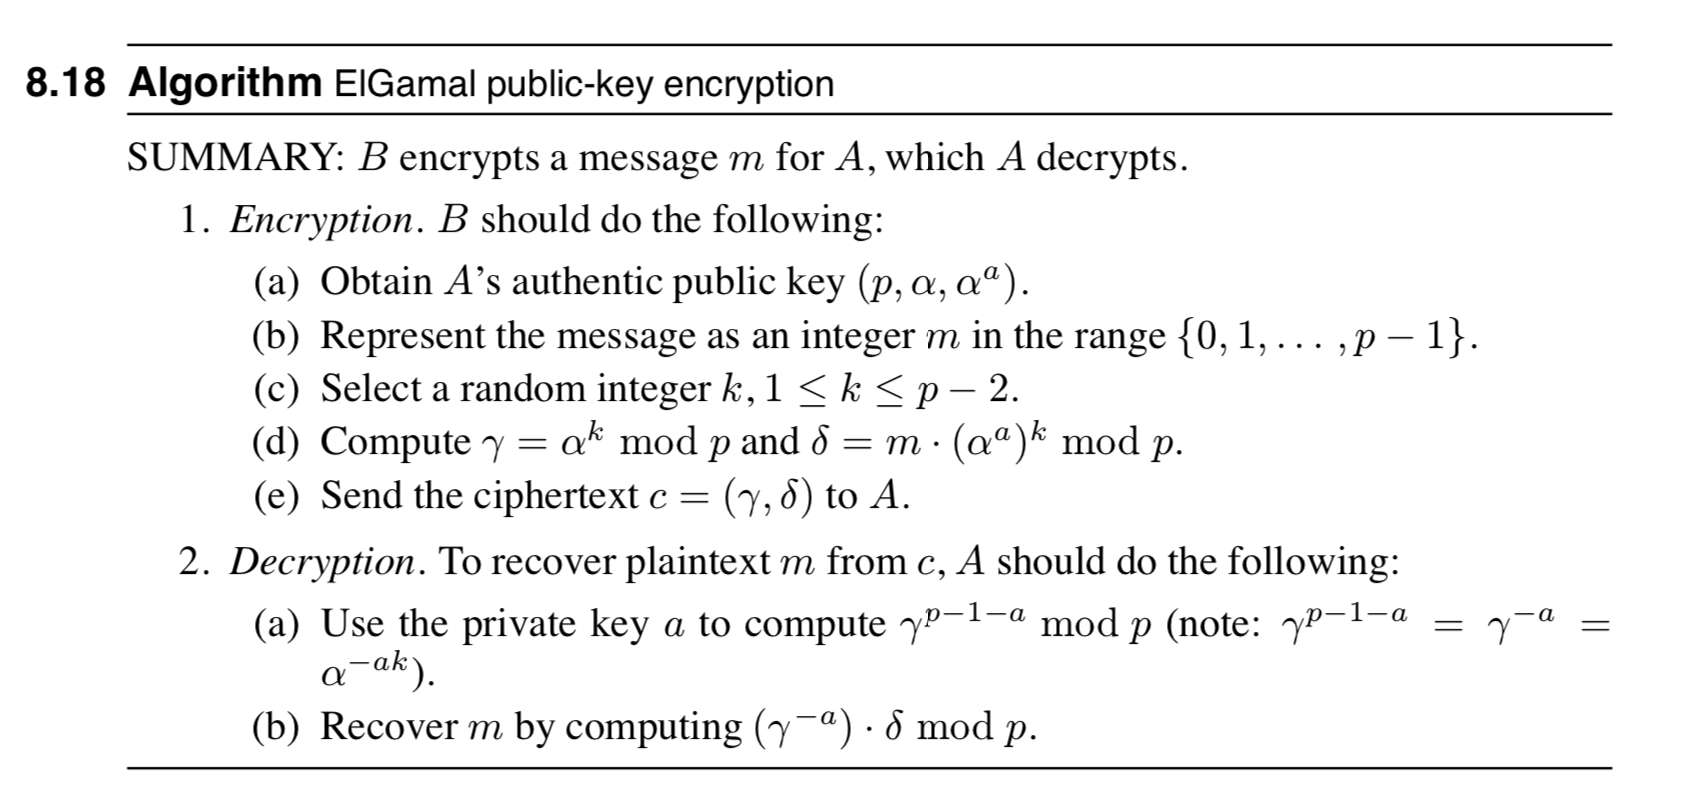
\includegraphics[width=0.9\textwidth]{assets/1f.png}
\end{figure}

Para agililizar las cuentas y descrifrar el texto más rápido, se hizo un \textit{script} en Python para
descifrar el texto:
\begin{minted}{python}
gamma = 54539

mensaje = [[(gamma, 81315,), (gamma, 87570,)],
           [(gamma, 31275,), (gamma, 35473,)],
           [(gamma, 25020,)],
           [(gamma, 18765,), (gamma, 50040,)],
           [(gamma, 31275,), (gamma, 50040,)],
           [(gamma, 12510,)],
           [(gamma, 50040,), (gamma, 68805,)]]

# Llave privada `a`
a = 137
# Z_p
p = 89627

def descifra_elgamal(g, d, a, p):
    # \gamma^{p-1-a} = \gamma^{-a}
    gamma_inv_a = pow(g, p - 1 - a, p)
    # (\gamma) \cdot \delta mod p
    m = pow(gamma_inv_a * d, 1, p)
    return m

# Cadena para guardar el texto descigrado
s = ''
# Iterar la lista
for l in mensaje:
    # Iterar las tuplas
    for t in l:
        # Tomamos la posición 0 y 1 de la tupla porque corresponden
        # a gamma y delta respectivamente.
        num_letra = descifra_elgamal(t[0], t[1], a, p)
        # Se hace un mapeo del número resultante al alfabeto
        s += chr(num_letra + 65)

# Texto descifrado
print(s)

\end{minted}
Dando como resultado el texto descifrado:
$$NOFUEDIFICIL$$

\end{enumerate}
%%%%%%%%

%%%%%%%%
\section{Sea $n = 4633$}

\begin{enumerate}[label=\alph*)]
\item Descomponer $n$ con el algoritmo de la criba cuadrática.\\
\sol Antes de proceder con el algoritmo, mostraremos el algoritmo y unas definiciones que serán usadas.\\
Decimos que un número es liso (\text{smooth number} en inglés) si se factoriza en número enteros
\textit{pequeños}. Por ejemplo un número $7$-\textit{smooth} es un número cuyos factores
son a lo más $7$ como $49=7^2$.\\
La fórmula explícita de símbolo de Lagrange es la siguiente: 
$$(\frac{a}{p}) \equiv a^{\frac{p-1}{2}} \pmod{p} \quad \and \quad (\frac{a}{p}) \in \{-1,0,1\}$$

\begin{figure}[h]
\caption{Algoritmo de la criba cuadrática}
\centering
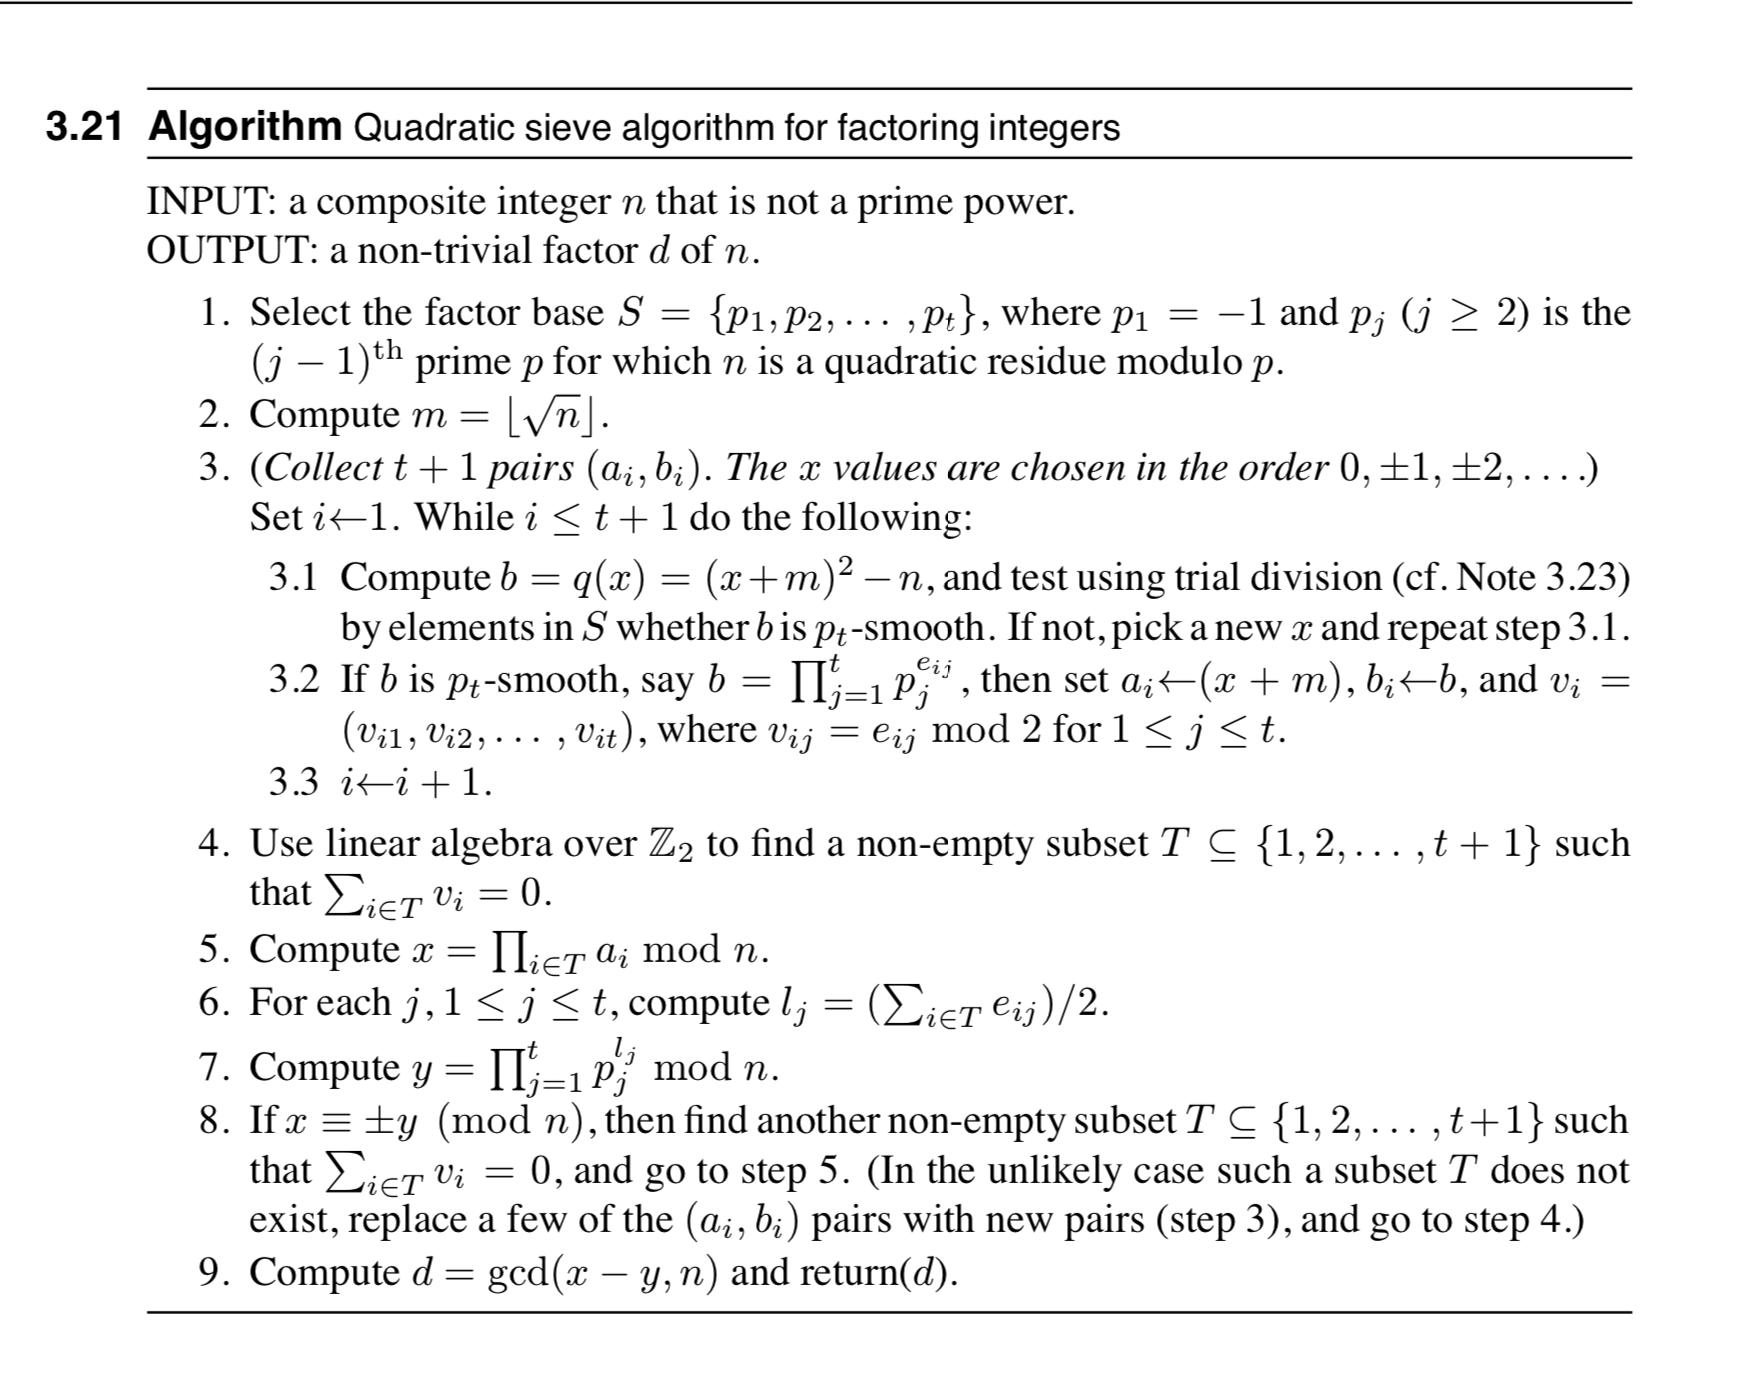
\includegraphics[width=0.9\textwidth]{assets/quadratic_sive.png}
\end{figure}

Ejecución del algoritmo.
\begin{itemize}
\item [1.] Tomamos $S = \{-1,2,3,17,19,29\}$\footnote{Se calculó cada dígito con la ayuda de esta
página web \url{https://adrianstoll.com/number-theory/jacobi.html} (bien se pudo programar pero 
se encontró más rápido de hacer con ésa herramienta).} de tamaño $t = 6$ porque según el algoritmo se 
toman los que $(\frac{n}{p}) = (\frac{4633}{p}) = 1$.
\item [2.] Calculamos $m=68$.
\item [3.] Se hace una tabla con los $t+1$ valores de $x$ para los cuales $q(x)$ es $29$-liso.
\begin{table}[h!]
\centering

\begin{tabular}{|l|l|l|l|l|l|}
\hline
$i$ & $x$ & $q(x)$ & Factorización de $q(x)$     & $a_i$ & $v_i$         \\ \hline
1   & 0   & -9     & $-2^3$                      & 68    & (1,0,0,0,0,0) \\ \hline
2   & -1  & -144   & $-2^4 \cdot 3^2$            & 67    & (1,0,0,0,0,0) \\ \hline
3   & 1   & 128    & $2^7$                       & 69    & (0,1,0,0,0,0) \\ \hline
4   & -3  & -408   & $-2^3 \cdot 3 \cdot 17^1$   & 65    & (1,1,1,1,0,0) \\ \hline
5   & 3   & 408    & $2^3 \cdot 3^1 \cdot 17^1$  & 71    & (0,1,1,1,0,0) \\ \hline
6   & 4   & 551    & $19 \cdot 29$               & 72    & (0,0,0,0,1,1) \\ \hline
7   & 5   & 696    & $2^3 \cdot 3 \cdot 29$      & 73    & (0,1,1,0,0,1) \\ \hline
\end{tabular}
\end{table}    

\item [4.] Tomando $T= \{v_1 + v_2\}$ tales que $v_1 + v_2= 0$.
\item [5.] Calcular $x = (a_1 a_2 \mod n) = 4489$.
\item [6.] Calcular $l_1=1$, $l_2=2$, $l_3=2$, $l_4=0$, $l_5=0$, $l_6=0$.
\item [7.] Calcular $y = -2^2 \cdot 3^2 = -36$
\item [8.] Como $4489 \not\equiv \pm 36 \pmod{n}$.
\item [9.] Entonces calculados el mínimo común múltiplo $gcd(x-y,n) = gcd(4592, 4633) = 41$.
Por tanto $4633$ tiene dos factores no triviales que son $41$ y $113$.
\end{itemize}


\item Cálcular $\phi(n)$ y descomponerla como producto de potencias de primos.\\
\sol Recordando de definción de la función aritmética $\phi$ que es:
$$\phi(n) = n \prod_{p \mid n} (1 - \frac{1}{p})$$
Como por el inciso anterior sabemos que $n=4633$ es un número compuesto de la forma
$n=41 \cdot 113$ podemos utilizar la definición de $\phi$.\\
Con ayuda de \textit{Python} se creo un programa para calcular $\phi(n)$,
\begin{minted}{python}
# Para mejor manejo de números racionales
from fractions import Fraction


def phi(n, factores_primos):
    # Incializamos el resultado con el valor de `n`
    r = Fraction(n, 1)
    # Iteramos sobra cada valor primo y lo multiplicamos 
    # según la definición de phi
    for p in factores_primos:
        r *= (1 - Fraction(1, p))
    # Como es un entero, regresamos el numerador
    return r.numerator

# Número al que se le aplicara la phi
N = 4633
# Lista de factores de N
L = [41, 113]

# Phi de Euler
print(phi(N, L))

\end{minted}
Ergo $\mathbf{\phi(n) = 4480}$.\\


Para encontrar la descomposisción de primos de $\phi(n)$ primero se hizo un analisis
previo con Factor\footnote{Un programa incluido en los binarios en la mayoría de las distribuciones Linux 
que dado un número lo descompone en primos. Para más información ver la siguiente 
página web \url{https://www.howtoforge.com/linux-factor-command/}} y se percató que sus factores primos no
son muy grandes, para evitar \textit{repercusiones} en la calificación de esta tarea se procedió a
realizxar un programa que realizará la factorización en primos del número.

\begin{minted}{python}
# Para mejor manejo de nímeros racionales
from fractions import Fraction

# Lista de los primeros 6 primos
primos = [2, 3, 5, 7, 11, 13]

def descoposicion_primos(N):
    factores_primos = []
    for p in primos:
        # Verificar si el número primo en turno es factor del número
        if N % p == 0:
            # Potencia del primo
            e = 1
            # Se Verifica hasta que potencia del primo divide al número
            while N % pow(p, e) == 0:
                # Se agrega el factor primo
                factores_primos.append(p)
                e += 1
    return factores_primos
    
N = 4480
print(descoposicion_primos(N))

\end{minted}
Una vez hecho el \textit{script} previo, se puede apreciar que los factores primos son los siguientes:
$$[2, 2, 2, 2, 2, 2, 2, 5, 7]$$
Ergo la descomposición en producto de primos queda como:
$$\phi(n) = 4480 = 2^7 \cdot 5^1 \cdot 7^1$$


\item Mostrar que $(11, \phi (n - 1)) = 1$.\\
\sol Teniendo $\phi(n-1) = \phi(4632)$, se procederá a obtener sus factorización canónica en primos para después
aplicar la definición de la función aritmética de phi de Euler. Como $4623 = 2^3 \cdot 3 \cdot 193$, 
utilizando el programa previamente hecho en el inciso $2b)$ se tiene que $\phi(4632) = 1536$.\\
Ahora para exhibir que $11$ y $1536$ son primos relativos, se deberan ver sus dividores y por definición 
deben de tener al $1$ como único factor común. Siendo $11$ un primo y $1536$ un número compuesto de la 
forma $1536 = 2^9 \cdot 3$. Ergo, el único número que los divide es $1$.


\item Encontrar $d$ tal que $d(11) \cong 1 \mod{(\phi(n - 1))}$.\\
\sol Recordando de definción de la función aritmética $d$ que es:
$$d(n) = \sum_{d \mid n} 1$$
Sea $n$ la descomposición canónica de un número, podemos descomponerlo de la siguiente manera
$d(n) = \prod_{i=1}^{k} p_i^{e_i}$. Como $11$ ser un número primo podemos aplicar la función 
aritmetica quedando de la forma $d(11) = (e_1 +1) = 1+1 = 2$.\\
Quedando la congruencia de la siguiente forma (recordando que $\phi(n-1) = \phi(4632) = 1536$):
$$2 \cong 1 \mod{1536}$$

\item Si la llave pública es $(n,11)$ descifrar el siguiente mensaje:
\begin{lstlisting}
930
1439
3707
484
2048
484
1093
\end{lstlisting}
\sol Teniendo calculado previamente $\phi(4633) = \phi(41)\phi(113) = 40 \cdot 112 = 4480$ Se procederá
con la ejecución del algoritmo.
\begin{itemize}
    \item $n=4633= 41 \cdot 113$.
    \item Calcular $\phi(4633) = 4480$.
    \item Nos dan $e=11$ como parámetro de nuestra llave pública, lo único es que se debe corroborar
    que $(4633,e) = (4633, 11) = 1$ (lu cual es verdad).
    \item Encontrar una $d$ (llave privada) tal que se satisfaga la siguiente congruencia 
    $de \cong 1 \mod{\phi(n)}$ que sustituyendo queda de la forma
    $d11 \cong 1 \mod{4480}$ que con ayuda de un programa\footnote{http://www.a-calculator.com/congruence/}
    se determinó dando $d=2851$.
    \item Sea $d=2851$.
\end{itemize}
Hecho el análisis previo, y teniendo la llave privada $d$, se sigue que $n=4633$ y $d=2851$. Ahora
se debe seguir la función de decifrado que es:
$$m = c^d \mod{n}$$
Con ayuda de un programa en \textit{Python} se hizo la exponenciación modular, que su forma de empleo
se traduce como $f(x,e,m) = x^e \mod{m}$
\begin{minted}{python}
def f(x, e, m):
    X = x
    E = e
    Y = 1
    while E > 0:
        if E % 2 == 0:
            X = (X * X) % m
            E = E / 2
        else:
            Y = (X * Y) % m
            E = E - 1
    return Y
\end{minted}
Sabiendo eso, se tiene que aplicar la función a cada renglón del mensaje, igual con ayuda de Python

\begin{minted}{python}
l = [930,1439,3707,484,2048,484,1093]

m = [f(x, 2851, 4633) for x in l]
\end{minted}
Dando $m = [5, 4, 11, 8, 2, 8, 3]$ haciendo un mapeo a cada letra del alfabeto indicando su posición 
$[0 \rightarrow A] ... [25 \rightarrow z]$ se tiene que el mensaje descifrado es:
$$\text{FELICID}$$


\end{enumerate}


%%%%%%%%
\section{Ejercicio 3}

\begin{enumerate}[label=\alph*)]
\item Mostrar que el problema del logaritmo discreto no depende del generador.\\
\sol Sea $\alpha$ and $\gamma$ dos generadores de un grupo cíclico $G$ de orden $n$, 
y sea $\beta \in G$. Sea $x=\log_a \beta$, $y=\log_\gamma \beta$, y $z = \log_\alpha \gamma$.
Entonces $\alpha^x = \beta = \gamma^y = (\alpha^z)^y$. Por consiguiente $x = zy \mod{n}$, y 
$$\log_\gamma \beta = (\log_\alpha \beta)(\log_\alpha \gamma)^{-1} \mod{n}$$
Esto significa que cualquier algoritmo de que calcule logarítmos a una base $\alpha$ puede ser
usado para calcular logaritmos a cualquier otra base $\gamma$ que también es un generador de $G$.

\item Sea $n = 10942095573514557503$ decir si es primo o compuesto en caso de ser
compuesto descomponerlo. (usando métodos vistos en clase).\\
\sol Usando el algoritmo de la criba cuadrática se procederá a factorizar el número.
Gracias a la ayuda del ayudantede laboratorio que nos proporcionó\footnote{
\url{https://github.com/kanekko/cryptography-and-security/blob/master/Lab07_Quadratic\%20Sieve/QuadraticSieve.java}}
y explicó el código en clase el código de éste, se utilizará para realizar su factorización y determinar si es
compuesto. Después de ejectutar el código, vimos que el número es compuesto de la forma:
$$10942095573514557503 = 23 \cdot 494664743 \cdot 961748927$$

\end{enumerate}
%%%%%%%%

%%%%%%%%%%%%%%%%%%%%%%%%%%%%%%%%%%%%%%%%%%%%%%%%%%%%%%%%%%%%%%%%%%%%%%%%%%%%%%%%%%%%%%%%%


%%%%%%%%%%%%%%%%%%%%%%%%%%%%%%%%%%%%%%%%%%%%%%%%%%%%%%%%%%%%%%%%%%%%%%%%%%%%%%%%%%%%%%%%%
\begin{thebibliography}{}

\bibitem{}
Alfred J. Menezes, Scott A. Vanstone, and Paul C. Van Oorschot. 1996.
\textit{Handbook of Applied Cryptography (1st ed.).}
CRC Press, Inc., Boca Raton, FL, USA.

\bibitem{}
Smooth number
\url{https://en.wikipedia.org/wiki/Smooth_number}

\bibitem{}
Notas tomadas en clases, ayudantías y laboratorio.

\bibitem{}
RSA Algorithm
\url{https://simple.wikipedia.org/wiki/RSA_algorithm}

\bibitem{}
Generators
\url{https://crypto.stanford.edu/pbc/notes/numbertheory/gen.html}


\end{thebibliography}
%%%%%%%%%%%%%%%%%%%%%%%%%%%%%%%%%%%%%%%%%%%%%%%%%%%%%%%%%%%%%%%%%%%%%%%%%%%%%%%%%%%%%%%%%

\end{document}
